\documentclass[../main/main.tex]{subfiles}
\graphicspath{{./figures/}}

\makeatletter
\renewcommand{\@chapapp}{Travaux pratiques -- TP}
\renewcommand{\chaplett}{TP}
\makeatother

% \toggletrue{student}
% \toggletrue{corrige}
% \renewcommand{\mycol}{black}
% \renewcommand{\mycol}{gray}

\hfuzz=5.003pt

\begin{document}
\setcounter{chapter}{1}

\settype{enon}
\settype{solu_prof}
\settype{solu_stud}

\chapter{\cswitch{%
	  Correction du TP
  }{%
	  Formation et observation d'images \`a distance finie~: mesures de distances%
  }%
 }%

\enonce{
	\begin{tcn}*(exem)<ctb>"how"'t'{Capacités exigibles}
		\begin{itemize}
			\item Mesure de longueurs sur un banc d'optique.
			\item Mettre en œuvre une mesure de longueur par déplacement du viseur
			      entre deux positions.
			\item Utiliser un viseur à frontale fixe, une lunette auto-collimatrice.
			\item Utiliser des vis micrométriques et un réticule pour
			      tirer parti de la précision affichée de l'appareil utilisé.
		\end{itemize}
	\end{tcn}

	\section{Objectifs}

	\begin{itemize}
		\item Réaliser des alignements sur un banc optique~;
		\item Reconnaître rapidement une lentille convergente et une lentille
		      divergente~;
		\item Déterminer une distance focale par différentes méthodes.
	\end{itemize}

	\section{S'approprier}

	\subsection{Principe de fonctionnement d'un viseur à frontale fixe}

	\noindent
	\begin{minipage}[c]{.48\linewidth}
		Un viseur à frontale fixe est constitué~:
		\begin{itemize}
			\item d'un objectif
			\item d'un réticule
			\item d'un oculaire
			\item d'une vis micrométrique permettant de translater le réticule selon un
			      axe orthogonal à l'axe optique.
		\end{itemize}
		L'objectif forme l'image A'B' de AB dans le plan focal objet de l'oculaire,
		tel que l'image finale est à l'infini, permettant pour l'œil une observation
		sans accommodation. Le réticule est dans ce même plan et est donc visible
		simultanément à l'objet AB. Globalement, le système peut être représenté par
		trois lentilles minces convergentes (dont le cristallin de l'œil) selon
		\[
			\rm AB
			\opto{\Lc_1}{\text{objectif}}
			A_1B_1
			\opto{\Lc_2}{\text{oculaire}}
			\underbracket[1pt]{\rm A'B'}_{\infty}
			\opto{\Lc_3}{\text{cristallin}}
			\text{image rétine}
		\]
	\end{minipage}
	\hfill
	\begin{minipage}[c]{.48\linewidth}
		\vspace{0pt}
		\begin{center}
			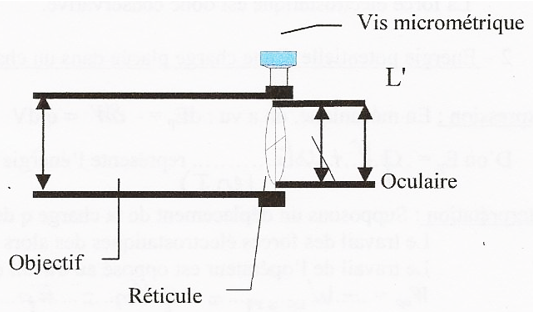
\includegraphics[width=\linewidth]{dispositif}
			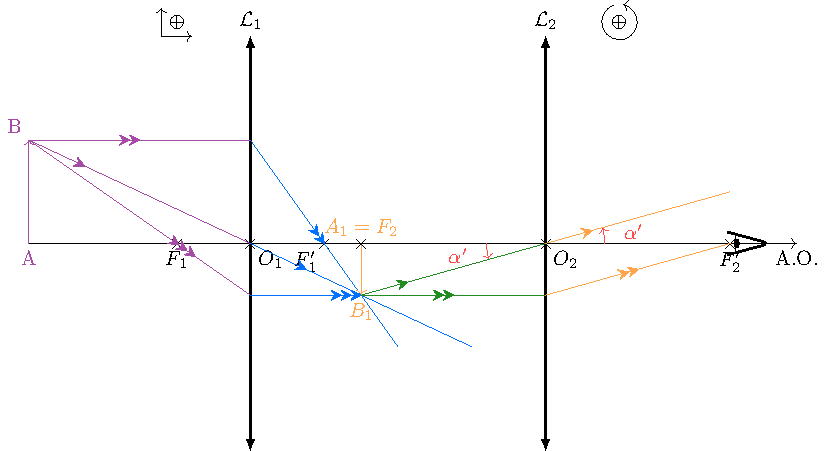
\includegraphics[width=\linewidth]{microscope}
		\end{center}
	\end{minipage}
	% \bigbreak
	% L'objectif forme l'image A'B' de AB dans le plan focal objet de l'oculaire,
	% tel que l'image finale est à l'infini, permettant pour l'œil une observation
	% sans accommodation. Le réticule est dans ce même plan et est donc visible
	% simultanément à l'objet AB. Globalement, le système peut être représenté par
	% trois lentilles minces convergentes (dont le cristallin de l'œil) selon

	% \[
	% 	\rm AB
	% 	\opto{\Lc_1}{\text{objectif}}
	% 	A_1B_1
	% 	\opto{\Lc_2}{\text{oculaire}}
	% 	\underbracket[1pt]{\rm A'B'}_{\infty}
	% 	\opto{\Lc_3}{\text{cristallin}}
	% 	\text{image sur la rétine}
	% \]

	% \begin{center}
	% 	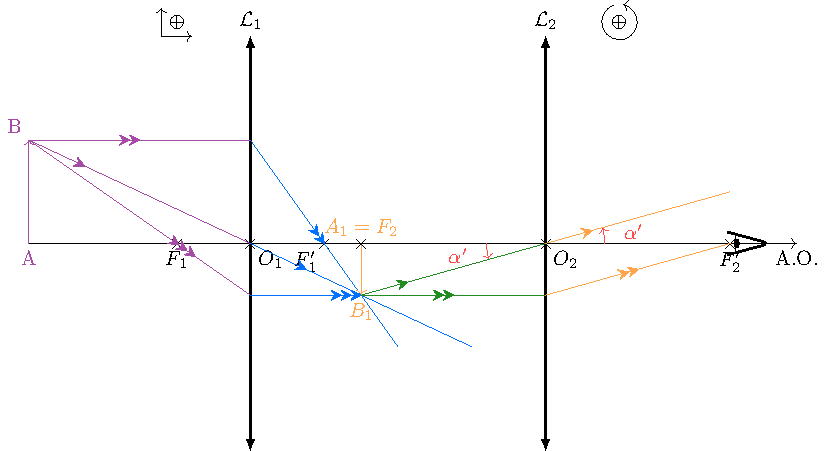
\includegraphics[width=.7\linewidth]{microscope}
	% \end{center}

	\begin{tcn}(impl)"bulb"{À comprendre}
		Un réticule est placé dans le plan focal objet de l'oculaire. Ainsi, il
		convient de translater le viseur sur le banc optique par rapport à l'objet
		pour voir simultanément l'objet et le réticule net. Nous noterons $D$ la
		distance séparant le centre optique de l'objectif de l'objet visé AB.
		Cette distance est fixe, ce qui explique la dénomination de viseur à
		frontale fixe.
	\end{tcn}
}

\setcounter{section}{2}
\setcounter{subsection}{1}
\subsection{Principe de lecture d'une vis micrométrique}

\enonce{
	La vis micrométrique permet de déplacer un double fil vertical dans le plan du
	réticule. La vis a un pas (translation réalisée pour un tour complet) de
	\SI{0.5}{mm} qui correspond à 50 graduations du tambour. On peut ainsi en
	déplaçant le fil vertical du réticule, mesurer la dimension de l'image A'B'
	réalisée de l'objet AB au \SI[parse-numbers=false]{1/100}{mm}.

	\begin{figure}[h]
		\centering
		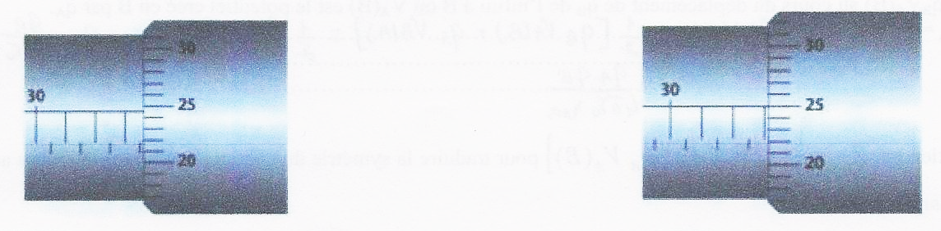
\includegraphics[width=0.7\linewidth]{vis_micro}
		\captionsetup{justification=centering}
		\caption{Principe de lecture sur une vis micrométrique. Un tour complet
			correspond à $\SI{0,5}{mm}$.}
		\label{fig:vis_micro}
	\end{figure}

	La lecture de gauche donne : $33+\num{0,5}+\num{0,245} = \SI{33,745}{mm}$.\\
	La lecture de droite donne : $33+\num{0,250} = \SI{33,250}{mm}$.
}

\setlist[blocQR,1]{leftmargin=10pt, label=\clenumi}

\QR{%
	Quelle est l'incertitude-type sur une telle mesure~? (s'aider de la
	fiche pratique sur la théorie de la mesure).
}{%
	Une graduation valant \SI{0.01}{mm}, on a une incertitude type B égale à une
	graduation sur racine de 3, soit
	\[
		u(x) = \frac{\Delta}{\sqrt{3}} = \SI{0.0058}{mm}
	\]
}

\enonce{
	\subsection{Principe de réalisation d'un pointé longitudinal avec un viseur}

	On cherche à déterminer la distance algébrique longitudinale $d = \obar{\rm
			AA'}$ dans la situation du schéma suivant.
	La mesure se déroule en deux étapes~:
	\begin{tcb}(expe)<itc>{Réglage du viseur}
		Translater l'oculaire en agissant sur l'œilleton de l'oculaire afin de mettre
		au point le réticule (c'est-à-dire voir les fils croisés nets).
	\end{tcb}

	\begin{tcn}(rema)<lftt>{Remarque}
		Ce réglage dépend de chacun, aussi il faut donc en théorie le réaliser à
		chaque fois que l'observataire change. En pratique, si votre œil est sans
		défaut, ou si ces défauts ont été corrigés, il n'est pas nécessaire de
		modifier les réglages pour les membres d'un binôme.
	\end{tcn}

	\noindent
	\begin{minipage}[c]{.48\linewidth}
		\begin{tcb}(expe)<itc>{Pointé longitudinal}
			\begin{enumerate}
				\item Viser l'objet $\rm AB$ (viser signifie voir l'image nette de
				      l'objet à travers le viseur). L'abscisse du viseur est alors~:
				      \[
					      x_{v}({\rm AB}) = x_{\rm A}+D
				      \]
				\item Viser l'image $\rm A'B'$. On a alors
				      \[
					      x_{v}({\rm A'B'}) = x_{\rm A'}+D
				      \]
			\end{enumerate}

			On en déduit alors la distance $d = \obar{\rm AA'}$ comme étant~:
			\[
				x_{v}({\rm A'B'}) - x_{v}({\rm AB}) =
				(x_{\rm A'}+D) - (x_{\rm A}+D) = d
			\]
		\end{tcb}
	\end{minipage}
	\hfill
	% \begin{figure}[htbp]
	% 	\centering
	% 	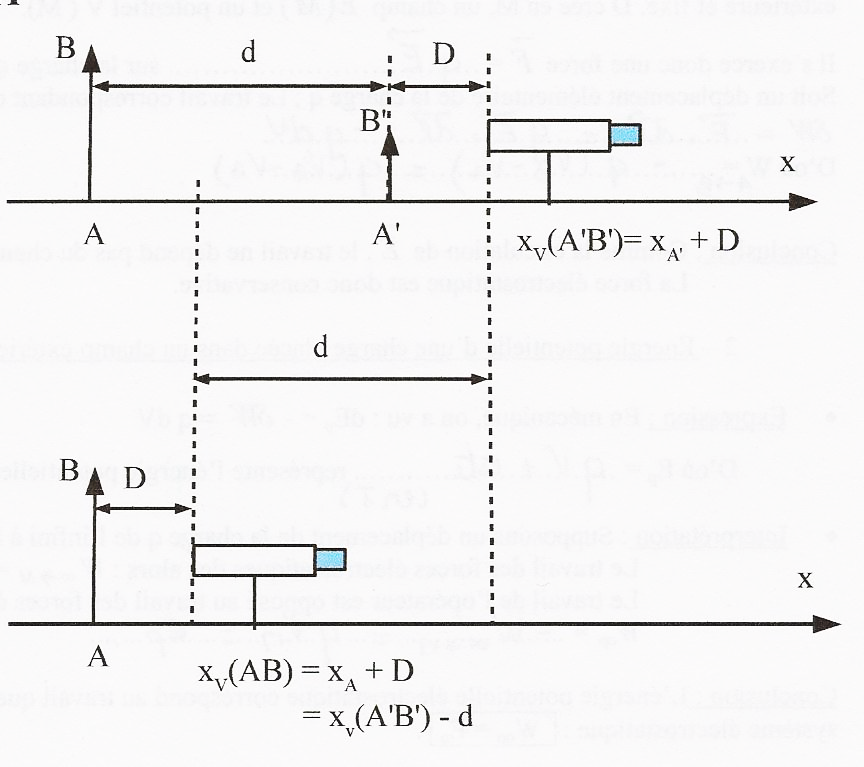
\includegraphics[width=.5\linewidth]{principe1}
	% \end{figure}
	\begin{minipage}[c]{.48\linewidth}
		\begin{center}
			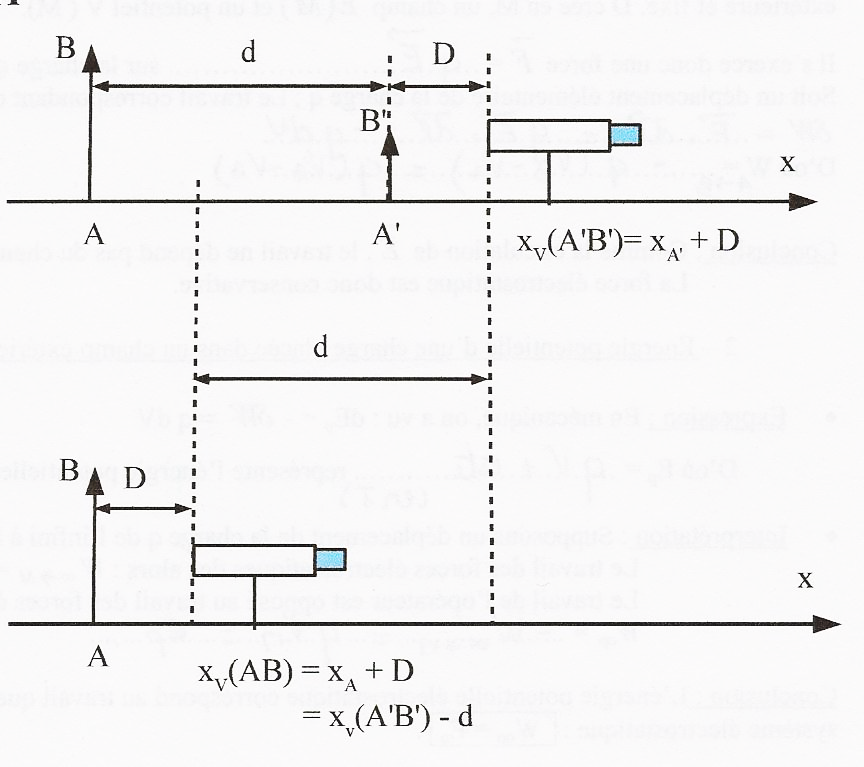
\includegraphics[width=\linewidth]{principe1}
		\end{center}
	\end{minipage}

	\subsection{Mesure du grandissement transversal du viseur}


	Le but de cette manipulation est de déterminer le grandissement
	transversal de l'\textbf{objectif} du viseur~: $\gamma = \ABp/\AB$. Pour
	cela, on détermine grâce à la vis micrométrique du viseur, la dimension de
	l'image A'B' d'un objet AB de dimension connue. L'objet AB de dimension connue
	est un micromètre, c'est-à-dire un axe gradué où 100 traits
	représentent $\SI{1}{cm}$. Le micromètre doit être horizontal.
	\begin{center}
		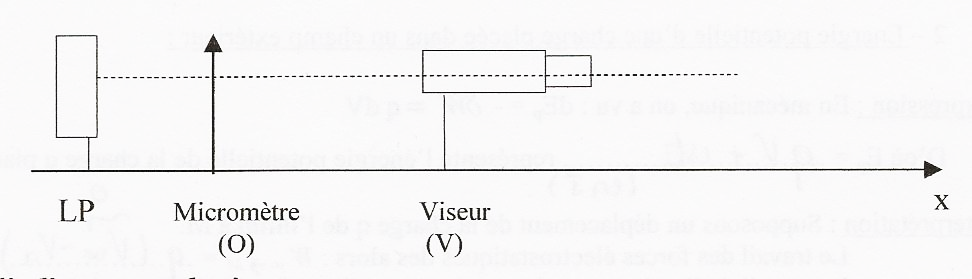
\includegraphics[width=\textwidth]{PointeTransversal}
	\end{center}

	\begin{tcb}[breakable](expe)<itc>{Pointé transversal}
		\begin{enumerate}
			\item Réaliser le montage ci-avant. Avant toute mesure, il faut régler
			      l'alignement des instruments d'optique.
			\item Approcher le viseur près du micromètre, vérifier les alignements des
			      instruments, puis s'en écarter tout doucement jusqu'à voir net le
			      micromètre dans le viseur en superposition avec le réticule.
			\item Grâce à la vis micrométrique, déplacer le fil vertical mobile du
			      réticule sur une graduation centrale du micromètre et noter
			      l'indication de la vis.
			\item Faire précisément 2 tours avec la vis micrométrique~: cela représente
			      un déplacement de $\SI{1}{mm}$ côté image.
			\item Relever, dans le viseur, la nouvelle graduation du micromètre pointée
			      par le fil vertical mobile.
			\item Déduire de ces relevés la valeur absolue du grandissement
			      $\abs{\gamma}$ de l'objectif du viseur.
			\item Sachant que l'objectif du viseur est constitué d'une lentille
			      convergente, en déduire le grandissement algébrique $\gamma$ de
			      l'objectif du viseur.
		\end{enumerate}
	\end{tcb}
}

\setcounter{subsection}{4}
\subsection{Focométrie~: rappel TP précédent (\textsc{Bessel} et
	\textsc{Silbermann})}
\enonce{%
	\begin{tcn}(rapp){Rappel}
		La focométrie consiste à déterminer expérimentalement la distance focale
		d'une lentille $(\Lc)$ inconnue.
	\end{tcn}

	\noindent
	\begin{minipage}[t]{.6\linewidth}
		À l'aide d'une lentille mince convergente $(\Lc)$ de distance focale
		image $f'$ inconnue, on veut former l'image d'un objet réel sur un écran
		situé à une distance $D$ de l'objet. En déplaçant la lentille, on trouve
		deux positions O$_1$ et O$_2$ qui donnent une image nette sur l'écran (cf.\
		figure ci-contre) à condition que $D \geq 4f'$. On a vu qu'alors la focale
		image $f'$ pouvait s'écrire~:
		\[
			f' = \dfrac{D^2-d^2}{4D}
		\]
	\end{minipage}
	\hfill
	\begin{minipage}[t]{.38\linewidth}
		~
		\begin{center}
			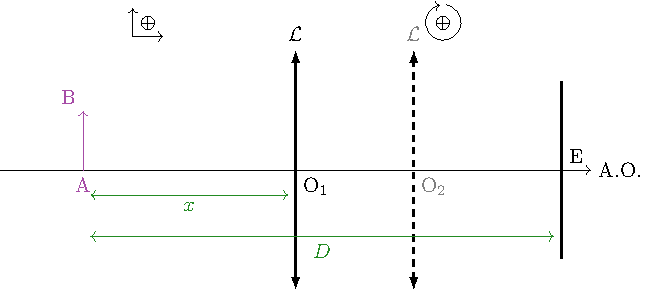
\includegraphics[width=\linewidth]{lent_conv-condition_bessel}
		\end{center}
	\end{minipage}

	La méthode de \textsc{Silbermann} est le cas particulier où $x_1 = x_2$.
}%
\QR{%
	Rappeler le protocole de la méthode de \textsc{Silbermann}.
}{%
	On détermine $f'$ en trouvant une unique position telle qu'il y ait une
	image nette.
	\smallbreak
	Pour cela, on commence avec $D$ grand et on cherche 2 positions
	nettes, et on réduit progressivement $D$ jusqu'à n'en avoir plus
	qu'une. On relève la plage de validité de $D$, on prend la valeur
	centrale et l'incertitude-type sera la demi-largeur de l'intervalle
	divisée par $\sqrt{3}$.
	\smallbreak
	On calcule alors $f' = \frac{D}{4}$ et $u(f') = \frac{u(D)}{4}$.
}

\section{Réaliser et valider}

\enonce{%
	Notebook \texttt{Capytale}
	disponible\ftn{\url{https://capytale2.ac-paris.fr/web/c/8e2d-1856963}}.
}%

\subsection{Pointé longitudinal}

\enonce{%
	Pour cette mesure, l'objet $\rm AB$ est constitué par la lettre $F$ et l'objet
	$\rm A'B'$ par un quadrillage dessiné sur feuille transparente. On séparera les
	deux objets d'une quinzaine de centimètres. On éclaire l'ensemble avec la
	lanterne (en $\SI{6}{V}$ alternatif) devant laquelle on interpose un écran
	dépoli pour limiter le flux lumineux.
}%

\resetQ
\setlist[blocQR,1]{leftmargin=10pt, label=\sqenumi}
\QR{%
	Suivre le protocole permettant de réaliser un pointé longitudinal et
	\textbf{valider} la méthode. Comparer pour ce faire la distance
	obtenue par pointé avec le viseur à la distance réelle entre les deux
	objets (lue directement sur le banc optique). Déterminer les
	incertitudes relatives, et en déduire l'écart normalisé.
}{%
	On trouve avec le viseur~:
	\begin{gather*}
		x_v(A) = \SI{27.500 \pm 0.058}{cm}
		\qet
		x_v(A') = \SI{42.100 \pm 0.058}{cm}
		\\
		\text{soit} \qquad
		\xul{d_v = \SI{14.600 \pm 0.082}{cm}}
		\qav
		u(d_v) = u(x_v) \sqrt{2}
	\end{gather*}
	et par lecture directe sur le banc~:
	\begin{gather*}
		x_b(A) = \SI{14.000 \pm 0.058}{cm}
		\qet
		x_b(A') = \SI{29.200 \pm 0.058}{cm}
		\\
		\text{soit} \qquad
		\xul{d_b = \SI{15.200 \pm 0.082}{cm}}
		\qav
		u(d_b) = u(x_b) \sqrt{2}
	\end{gather*}
	Ainsi, on a un écart normalisé
	\begin{gather*}
		\boxed{E_N = \frac{\abs{d_b - d_v}}{\sqrt{u(d_b)^{2} + u(d_v)^{2}}}}
		\\
		\mathrm{A.N.~:}\enskip
		\xul{E_N = \num{0.73} < 2
		}%
		\\
	\end{gather*}
	Les deux mesures sont bien compatibles.
}%

\enonce{%
	\begin{tcn}(rema)<lftt>{Remarque}
		Évidemment, dans la situation
		présente, la méthode semble un peu artificielle, puisqu'il est possible de
		lire directement sur le banc optique la position des objets. Néanmoins, dans
		une situation plus réaliste, une telle méthode peut s'avérer très utile
		puisqu'il devient alors possible de déterminer de loin la distance séparant
		deux objets.
	\end{tcn}
}%

\subsection{Pointé transversal~: largeur d'un fil de cuivre}

\QR{%
	Réaliser la mesure du grandissement de l'objectif du viseur.
}{%
	Le réticule vu au travers du viseur pointe sur l'abscisse \num{50} du
	viseur, soit \SI{5}{mm}, avant l'opération sur la vis micrométrique.
	\smallbreak
	Après exactement deux tours, le réticule a physiquement été déplacé de
	\SI{1}{mm}. En lisant au travers du viseur, le réticule pointe
	maintenant sur l'abscisse \num{60}, soit \SI{6}{mm}. Ainsi, le
	grandissement de l'oculaire du viseur est $\abs{\gamma} =
		\frac{\ABp}{\AB} = 1$, avec $\ABp$ la taille de l'image vue au travers
	du viseur (donc le micromètre de \SIrange{5}{6}{mm}) et $\AB$ la
	distance réelle parcourue par le réticule (donc \SI{1}{mm}).
	\smallbreak
	Comme c'est une lentille convergente, l'image est forcément renversée
	(objet réel avant le foyer objet), donc techniquement $\gamma = -1$.
	\smallbreak
	On en conclue que le déplacement appliqué sur le réticule par la vis
	micrométrique est tout à fait le même au déplacement observé au
	travers du viseur~: on peut ainsi mesurer une épaisseur par
	visualisation au travers de celui-ci.
}%
\QR{%
	Prendre comme objet un fil de cuivre, le viseur, positionner
	correctement le fil vertical du réticule et, connaissant le
	grandissement de l'objectif du viseur, en déduire l'épaisseur de
	celui-ci.
}{%
	On place le réticule à gauche du fil de cuivre. On lit la position du
	réticule sur la vis micrométrique~: $x_{R,g} = \SI{4.5300 \pm
			0.0058}{mm}$.
	\smallbreak
	On déplace le réticule du côté droit du fil de cuivre. On lit la
	position du réticule sur la vis~: $x_{R,d} = \SI{5.5300 \pm
			0.0058}{mm}$. On a donc une épaisseur~:
	\[
		\boxed{e = \abs{x_{R,d} - x_{R,g}}}
		\Ra
		\xul{e = \SI{1.0000 \pm 0.0081}{mm}}
	\]
}%

%\subsection{\'Evaluation de la distance frontale du viseur}
%
%%\'Evaluer la distance focale de la lentille constituant le viseur, en mesurant la distance frontale $D$ (entre ce qu'on vise et le viseur) avec un réglet. Exprimer f' en fonction de ? et D. Faire l'application numérique.

\subsection{Relation de conjugaison de \textsc{Descartes}}

\enonce{
	\subsubsection{Montage}

	% \begin{wrapfigure}[4]{r}{0.62\textwidth}
	% 	\vspace*{-40pt}
	% 	\begin{center}
	% 		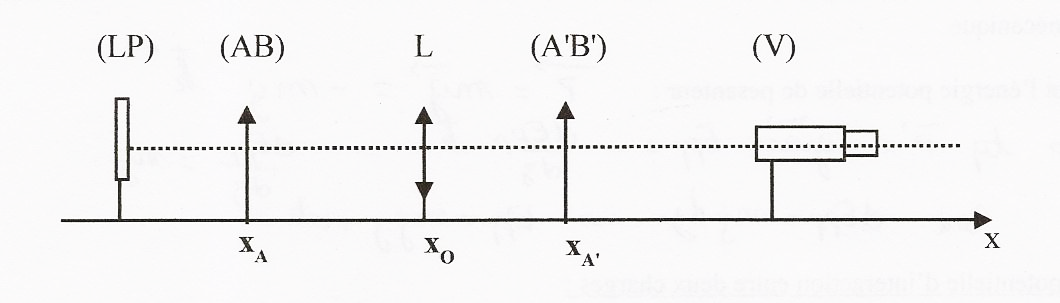
\includegraphics[width=0.6\textwidth]{pointeLongitudinal}
	% 	\end{center}
	% \end{wrapfigure}

	\noindent
	\begin{minipage}[c]{.48\linewidth}
		Prendre comme objet AB la plaque constituée des lettres $F$ sur papier
		translucide et réaliser le montage ci-contre avec une lentille convergente
		de la focale de votre choix.
	\end{minipage}
	\hfill
	\begin{minipage}[c]{.48\linewidth}
		\begin{center}
			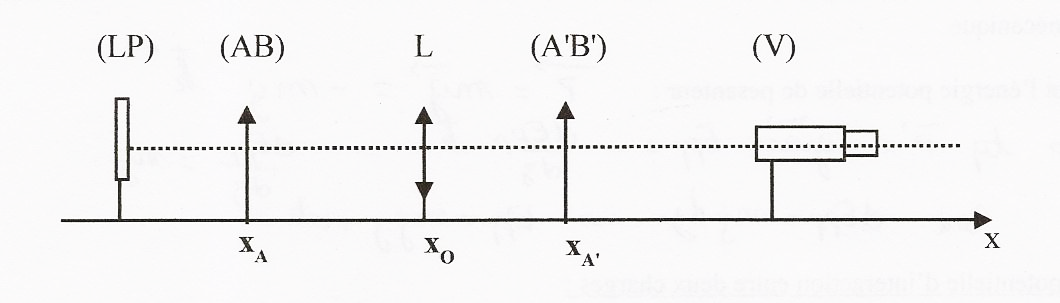
\includegraphics[width=\linewidth]{pointeLongitudinal}
		\end{center}
	\end{minipage}
}

\setcounter{subsubsection}{1}
\subsubsection{Mesures}

\enonce{
	\begin{tcb}[breakable](expe)<itc>{Relation de conjugaison}
		\begin{enumerate}
			\item Chercher la position approximative de l'image A'B' de AB ainsi
			      obtenue grâce à un écran.
			\item Viser ensuite cette image A'B' avec le viseur. Noter l'abscisse $x_1
				      = x_{\rm A'} + D$ du viseur sur le banc.
			\item Mettre un petit morceau de papier sur la lentille $\Lc$, viser
			      celle-ci avec le viseur en réalisant la mise au point sur les déchirures
			      du papier.
			\item Noter l'abscisse $x_2 = x_0 + D$ du viseur sur le banc.
			\item Viser enfin l'objet AB avec le viseur (après avoir ôté la lentille).
			\item Noter l'abscisse $x_3 = x_{A} + D$ du viseur sur le banc. Déduire
			      des mesures $\OA$ et $\OAp$ en fonction de $x_1$, $x_2$ et $x_3$.
		\end{enumerate}
	\end{tcb}
}

\QR{%
	Faire les applications numériques et à l'aide de la relation de conjugaison
	avec origine au centre des lentilles minces, calculer $f_{\rm desc}'$.
}{%
	En cours…
}%
\QR{%
	Estimez les incertitudes, puis calculer l'écart normalisé entre $f_{\rm
				desc}'$ et $f_{\rm th}'$ (distance focale indiquée sur la lentille).
}{%
	En cours…
}%

\subsubsection{Observation d'une image virtuelle}

\QR{%
	Proposer et réaliser un protocole permettant d'observer à l'aide du
	viseur une image virtuelle avec la lentille $V = -\SI{10}{\delta}$.
	Quelles sont les contraintes à respecter~? Faire constater votre montage
	(réussi) par la professeure.
}{%
	On place un objet contre une lampe suivi d'un écran dépoli sur un banc
	d'optique.
	\smallbreak
	On place une lentille de $V = -\SI{10}{\delta}$ devant l'objet.
	\smallbreak
	Pour observer l'image virtuelle obtenue, il faut que l'image en question soit
	visible avec le viseur dans l'espace image réelle de la
	lentille. Comme le viseur doit être décalé d'environ \SI{15}{cm} pour
	ça, l'image virtuelle doit être à moins de \SI{15}{cm} du centre de la
	lentille.
	\smallbreak
	On place alors le viseur après la lentille, en observant au-travers de
	celle-ci.
}%

\subsection{Focométrie par la méthode de \textsc{Bessel} avec un viseur}

\enonce{
	Le viseur joue alors le rôle de l'écran dans la méthode de \textsc{Bessel} telle
	que vue dans la partie théorique.

	\begin{tcb}(expe)<itc>{\textsc{Bessel} au viseur}
		\begin{enumerate}
			\item Fixer la position de l'objet AB.
			\item Pointer l'objet AB avec le viseur et noter $x_0$ l'abscisse du
			      viseur.
			\item Interposer la lentille $\SI{8}{\delta}$ entre l'objet et le viseur.
			\item Déplacer le viseur d'une distance $D > 4f'$ simple et facile à
			      repérer. L'abscisse du viseur est alors $x_0 + D$.
			\item Déterminer les positions de la lentille O$_1$ et O$_2$ qui réalisent
			      la conjugaison objet image en déplaçant la lentille entre l'objet et le
			      viseur, afin d'obtenir une image nette à travers le viseur. Relever les
			      deux positions correspondantes de la lentille notées $x_1$ et $x_2$.
		\end{enumerate}
	\end{tcb}
}

\QR{%
Calculer $d = x_2-x_1$, puis en déduire $f'_{\rm bess}$.
}{%
En cours…
}%

\QR{%
Appliquer la méthode de \textsc{Silbermann} pour obtenir $f'_{\rm silb}$ par
une autre méthode.
}{%
En cours…
}%

\QR{%
	Avec l'écart normalisé, comparer les valeurs de $f'$ obtenues
	expérimentalement par chacune des méthodes avec la valeur donnée sur la
	monture de la lentille, en estimant les différentes incertitudes.
}{%
	En cours…
}%

\end{document}
